\documentclass[10pt,a4paper,pointlessnumbers,bibtotocnumbered,headsepline]{scrbook}
\usepackage{longtable,tabularx}
%\usepackage{supertabular} 
\usepackage{afterpage}
\usepackage{verbatim}
\usepackage{fancybox}
\usepackage{makeidx}
\usepackage{afterpage}
%\usepackage[draft]{graphicx}
\usepackage{graphicx}
\usepackage{bigstrut}
\usepackage[small]{caption2}
\abovecaptionskip1.5mm
\belowcaptionskip5mm
\renewcommand{\captionfont}{\small\itshape}
\renewcommand{\captionlabelfont}{\bfseries}
\LTpost=\belowcaptionskip
\usepackage[colorlinks]{hyperref}

% palatino fonts are standard
% ---------------------------
\usepackage{palatino}

% listings
% --------
\usepackage{listings}
\lstloadlanguages{C}
\lstset{
  basicstyle=\scriptsize,
  keywordstyle=\bfseries,
  commentstyle=\slshape,
  stringstyle=\ttfamily, 
% RS: seems to have changed in newer LaTeX packets...
% labelstep=5,
% labelstyle=\tiny, 
% indent=20pt
}  

% paper format
% ------------
\usepackage{geometry}
\geometry{dvips, pdftex}
%\geometry{paperwidth=210mm}
%\geometry{paperheight=297mm}
%\geometry{top=12mm}
%\geometry{bottom=20mm}
%\geometry{textwidth=170mm}
%\geometry{left=20mm}
%\geometry{twosideshift=10mm}
%\geometry{headsep=0mm}
%\geometry{head=40mm}
%\geometry{footskip=12mm}

\evensidemargin0mm
\oddsidemargin0mm

% head- and footlines 
% -------------------

%\usepackage{fancyhdr}
%\usepackage{psboxit}
%%\renewcommand{\headrule}{\includegraphics{longline}}
%\renewcommand{\sectionmark}[1]{\markboth{\thesection #1 Bla}}
%\lhead[\sf Kapitel \thechapter]{\fancyplain{}}
%\rhead[\fancyplain{}]{\sf \rightmark}
%%\lfoot[\includegraphics{shortline}\\\sf\thepage]{\fancyplain{}}
%\lfoot[\rule{12mm}{0.5pt}\\\sf\thepage]{\fancyplain{}}
%%\rfoot[\fancyplain{}]{\includegraphics{shortline}\\\sf\thepage}
%\rfoot[\fancyplain{}]{\rule{12mm}{0.5pt}\\\sf\thepage}
%\cfoot{\fancyplain{}}


\raggedbottom

% PDF parameters
% \pdfcompresslevel=9


% please make me an index
\makeindex

% some spacings
\setlength{\parindent}{0 pt}
\setlength{\parskip}{0.5\baselineskip plus 2 pt minus 2 pt}
%\setlength{\parskip}{1.5ex plus 0.5ex minus 0.3ex}
\setlength{\baselineskip}{1\baselineskip plus 0pt minus 0pt}

% space on top and bottom of the page which can be used by floatingfigures 
\renewcommand{\topfraction}{0.7}
\renewcommand{\bottomfraction}{0.7}
\renewcommand{\floatpagefraction}{0.7}

% tolerance of the characters 
\tolerance=2000
\emergencystretch=20pt

% avoid Hurenkinder and Schusterjungen
\clubpenalty=9999\relax
\widowpenalty=9999\relax

% don't allow page breaks in footnotes 
\interfootnotelinepenalty=10000 


% headline 
%\pagestyle{fancyplain}


% environment for code samples 
% ---------------------------- 
\newenvironment{code}{\begingroup\verbatim}{\endverbatim\endgroup}
\newenvironment{smallcode}{\begingroup\footnotesize\verbatim}{\endverbatim\endgroup}


% for test purposes: make line on the baseline 
\newcommand{\HR}{\rule{1em}{.4pt}}

% itemize environment with less space 
\newenvironment{myitemize}{
  \begin{itemize}
    \setlength{\itemsep}{-3 pt}
    \setlength{\parsep}{0 pt}
}{
  \end{itemize}
}      


% exclamation mark environment
% ----------------------------
\newenvironment{important}{
  \vspace{1ex plus 1ex}
  \begin{minipage}[c]{\textwidth}
  
  \begin{center}
  \rule{0.99\textwidth}{2pt}

  \vspace{1ex}

  \begin{minipage}[c]{0.1 \textwidth}
    {\Huge \bf \sf \textcircled{\Large !}}
  \end{minipage}
  \begin{minipage}[c]{0.85 \textwidth}
    \begingroup\sf
}{
    \endgroup
  \end{minipage}

  \vspace{1ex}

  \rule{0.99\textwidth}{2pt}
  \end{center}
  \end{minipage}
  \vspace{1ex plus 1ex}
}

\hyphenation{make Named Linux}


%%%%%%%%%%%%%%%%%%%%%%%%%%%%%%%%%%%%%%%%%%%%%%%%%%%%%%%%%%%%%%%%%%%%%%%
\begin{document}
%%%%%%%%%%%%%%%%%%%%%%%%%%%%%%%%%%%%%%%%%%%%%%%%%%%%%%%%%%%%%%%%%%%%%%%

\newpage
\thispagestyle{empty}

\begin{center}
{
\Large \sf Robert~Schwebel 

\vspace{2 cm}

\Huge \sf \textbf{The PTXdist Manual}
}

\vspace{\fill}

{
\Large \sf \copyright \, 2004 by Pengutronix. All Rights Reserved. \\
All kind of duplication other than explicitly allowed is prohibited.
}

\end{center}

\newpage

% -----------------------------------------------------------------------------
\markboth{\sffamily\small\upshape\bfseries Table of Contents}{\sffamily\small
  \upshape\bfseries Table of Contents}
\markright{\sffamily\small Table of Contents}
\thispagestyle{headings}

{
\parskip0mm
\tableofcontents
}

% -----------------------------------------------------------------------------

\part{Introduction}
% ----------------------------------------------------------------------------
\chapter{Embedded Linux} 			\label{chap:embedded-linux}
% ----------------------------------------------------------------------------

\begin{flushright}
\emph{
If you treat your beta-testers as if they're \\
your most valuable resource, they will respond \\
by becoming your most valuable resource.\\
}
\textsc{\small Eric S. Raymond}
\end{flushright}

Once upon in time embedded systems didn't need operating systems. Things
have been so easy: all a developer needed was a good toolchain,
consisting of compilers and other development tools, probably an EPROM
burning device and things started working. After some time every
register of the CPU was known, a variety of library routines have been
developed and our brave developer was able to do his project with the
more and more well known system. The controllers had legacy interfaces
like RS232, i2c or SPI which connected them to the outside world and the
main difference between the controllers available on the marked was the
number of GPIO pins, UARTS and memory ressources. 

Over the time, things have changed. Hardware manufacturers have weakened
the border between microcontrollers --~devices meant to work in embedded
systems~-- and full blown microprocessors. Structures became much more
complicated: where our good old controllers had just some interrupts
with some small interrupt service routines we today need complicated
generic interrupt infrastructures, suitable for generic software
frameworks. Where we had some linearly mapped flash ROM and some data
RAM we today have multi-stage-pipeline architectures, memory management
units, virtual address spaces, on-chip-memory, caches and other
complicated stuff, which is not exactly what the embedded system
developer wants do every other day. 

Entering embedded operating systems. Although there are still some
processors out there (like the popular ARM7TDMI based SoCs) which can be
programmed the good old non-operating-system way, it is becomming more
and more difficult. On the other hand, legacy I/O interfaces like RS232
are increasingly replaced by modern plug-and-play aware communication
channels: USB, FireWire (IEEE1394), Ethernet \& friends are more and
more directly being integrated into today's microcontroller hardware.
Whereas some of these interfaces can "`somehow"' be handled the old
controller-style way of writing software, the developer following this
way will not be able to address the security and performance issues
which come up with the modern network accessable devices.

During the last years, this resulted in more and more of the small-scale
companies which developed little embedded operating system being pushed
out of the market. Nearly no small company is able to support all the
different interfaces, communication stacks, development tools and
security issues out there. New interfaces and -variants (like USB
on-the-go) are developed faster than operating system developers can
supply the software for them. This today results in a market
consolidation: only the largest commercial embedded operating system
supplyers will survive. 

Only the largest commercial...? There is one exception: when the same
situation came up in the "`mainstream"' computer market at the beginning
of the 1990ies, people started to develop an alternative to the large
commercial operating systems: Linux. Linux did never start with a
ready-to-use solution: people had a problem, searched for a solution but
didn't find one. Then they started to develop one themselves, often
several people did this in parallel, and in a huge community based
evolution mechanism the best solutions found their way into the Linux
kernel, which over the time formed one of the most reliable and
performant kernels available today. This "`develop-and-evolute"'
mechanism has shown it's effectiveness over and over again in the
server and desktop market today. 

Also for embedded systems Linux grew more and more popular. Studies have
shown that more than 70\% of the embedded developers are not satisfied
with a black box operating system: they want to adapt it to their needs,
to their special hardware situation (which most times is Just Different
than anything available). Embedded projects are even more variegated
than desktop- or server projects, due to the fact that there exist so
many different embedded processors with lots of peripherals out there.
Linux has evolved from a i386 only operating system to a kernel running
on nearly every modern 32 bit processor available today: x86, PowerPC,
ARM, MIPS, m68k, cris, Super-H etc. The kernel supplies a hardware
abstraction layer which lets our brave embedded developer once again
concentrate on his very special problem, not on handling neglibilities
like memory management. 

But Linux is only half of the story. Besides the kernel, a Linux based
embedded system consists of a "`Userland"': a filesystem, containing all
the small tools which form a small Unix system. Only the combination of
the kernel and a Userland let's the developer run "`normal"' processes
on his x86 development machine as well as on his embedded target. 

Whereas the mainstream developers were always able to use normal Linux
distributions like SuSE, RedHat, Mandrake or Debian as a base for their
applications, things are different for embedded systems. Due to the
restricted ressources these systems normally have, distributions had to
be small and should only contain that things which are needed for the
application. Additionally, they had to be auditable and reproducable:
Embedded developers usually want to know what's in their systems -- be
it that they have to support their software for a long time span
(something like 10-15 years are usual product lifetimes in automation
applications) or that they have such a special scenario that they have
to maintain their integrated source of their Userland themselves.
Entering PTXdist. 

% ----------------------------------------------------------------------------
\chapter{Maintaining Userlands} 		\label{chap:userlands}
% ----------------------------------------------------------------------------

\begin{flushright}
\emph{
Use the source, Luke!\\
}
\textsc{\small Obi-Wan Kenobi}
\end{flushright}

The idea for PTXdist came up when the people at Pengutronix had to
compile the userlands for customer projects over and over again. Nearly
no customer had the same requirements: one needed network tools like
\texttt{ifconfig}, servers like \texttt{thttpd} or \texttt{dhcpd},
others needed tools for accessing displays, embedded web browsers or
other Human Machine Interface stuff. 

The systems most time were so different that the way of stripping down a
mainstream distribution did not work well: you simply cannot strip down
a Debian system small enough to fit into a 2~MB RAM and 2~MB Flash
system without destroying the whole idea behind the distribution. The
other way is to build a Userland from scratch: Linux distributions like
LFS follow this path, but users have to do every configuration and
compilation step one after the other, which is a time consuming and
errorprone way. 

What we basically needed when we started PTXdist was: 
\begin{itemize}
\item A configuration frontend which lets the embedded developer just
      select which components he wants to have in his Userland. The
      configuration should be totally independend from the rest of the
      system. 
\item The system should be small at this time: no need to download
      several tens of megabytes from the net, even before selecting what
      would go into the image.
\item A set of rules, easily readable by every reasonably silled Unix
      develper, which reads the configuration and defines how to 
      build a certain software packet, taking into account what the 
      user has selected during configuration. 
\item A framework which makes it easy for a developer to add new packets
      to the system when he needs something which is not yet integrated. 
\item The whole thing should be Open Source like the Linux kernel and
      the Userland software itself, as our customers wanted a completely
      transparent, modificable and debuggable software framework, be it 
      the bootloader, the kernel or, finally, the Userland tools. 
\item Last but not least, the whole system should be platform
      independend, to build userland for whatever architecture the 
      user works with. 
\end{itemize}

When we looked around for existing solutions there was none that
fulfilled all these requirements: some where large beasts (like the
uClinux distribution), some had an interesting approach (like the
emDebian Project) but used the wrong tools (CML2 for configuration,
which is basically a dead project today), others had a great
infrastructure for the rules (like buildroot, part of the uClibc
project) but no configuration frontend usable by normal end users. So we
finally had a look at all the available projects, collected the best
ideas and started a new Open Source project: PTXdist. 

Over the last two years, PTXdist grew with the projects which have been
developed for Pengutronix' customers. PTXdist is still no distribution:
distributions are meant to just-work-out-of-the-box, which is simply not
possible for the multifaceted situations we have in embedded projects.
The idea behind PTXdist is more something like: 

\begin{important}
{\bf PTXdist is "`Executable Documentation"'. Write down what you 
did once to make something work, in a well defined manner, and
implicitly don't forget it until you need it the next time.}
\end{important}

When a Userland for a certain customer board is developed, the PTXdist
framework is used to document all the necessary steps to build the
binaries from the original sources. PTXdist defines which configuration
switches have to be selected, which tweaks have to be applied to buggy
upstream source trees and which are the commands which have to be
started in which order to build a working tree. 

At the end of a development project, the customer normally has a
standard configuration integrated in PTXdist which lets him build his
own Userland with \texttt{make~world}, he is able to work with the
framework and switch on and off things he wants to change himself. Some
customers have enough skills to send patches in case some randomly
switched on config button doesn't show the expected results, others use
Pengutronix' support services to integrate new packets into PTXdist or
fix problems which come up with configuration constellations which have
beed never tested before (with over 600 config entries there are $2^600$
possible combinations -- it would take some time to test them all). 

And, of course, we managed to build a community around PTXdist, which
consists mainly of a mailing list on the PTXdist server. People outside
Pengutronix started to work with the system for their own project, which
is very important to make PTXdist more robust and test it in
constellations which have not yet been realized here.  

So when you start your next Embedded Linux project with PTXdist don't
expect it to be something "`finished"' -- it is as finished or
unfinished as the Linux kernel itself, which is just a collection of
software which has proven to be great in one or the other situation, and
which has been looked over by several people. The more people use
PTXdist for their projects, the more robust and the more feature rich it
becomes -- just like with the kernel. The power of Linux and PTXdist
come from it's Open Source nature and from people working together to
form an industry quality software framework -- you just have to join the
team!



\part{End User Manual}
% ----------------------------------------------------------------------------
\chapter{Building Blocks of PTXdist} 		\label{chap:building-blocks}
% ----------------------------------------------------------------------------

\section*{The Big Picture}

PTXdist is good for basically two tasks: compiling stuff for an embedded
system, which means to compile components which go into the
\texttt{root/} directory of the PTXdist tree, and compiling tools which
are needed on the development host to build other code for the target. 

\begin{important}
The PTXdist manual does consequently talk about two computers you
usually work with: one is the \emph{development host} -- this is the
normal PC you work on. The development host needs a generic Linux
distribution (for example Debian, SuSE, RedHat or Mandrake).  The other
one is the \emph{embedded target}, sometimes also referenced as the
\emph{target}. The Target is usually an embedded device and may have
another processor architecture than your development host.
\end{important}

% -----------------
\begin{figure}[b]
	\centerline{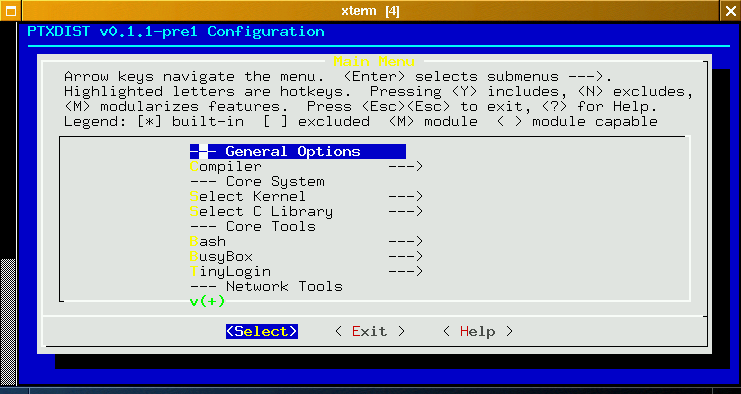
\includegraphics[width=0.99\textwidth]{figures/menuconfig}}
	\caption{
		KConfig in menuconfig mode: select what you want in your
		target. 	
		\label{fig:menuconfig}
	}
\end{figure}
% -----------------

Code for the host is being compiled with the distribution's native C
compiler (normally GCC), whereas you need a cross compiler to build code
for the target. We'll discuss later how you can get a cross compiler,
just in case you don't have one yet. 

Before we start digging deeper into PTXdist's internals let's have a
look at the building blocks the system consists of. The main building
blocks are: 

\begin{itemize}
\item The KConfig frontend (select what you want to have in your root
      filesystem), and
\item A set of Makefiles (rules which contain what has to be done).
\end{itemize}

The KConfig frontend is normally used by somebody who wants to configure
a \emph{selection} of programs which are later put into the root
filesystem of an embedded system; configuring mostly consists of
clicking on software components you want to install. Once you have a
working set of rules and a sane \emph{base} for your projects, you can
use the KConfig frontend to make your selection, without the need to do
further changes on a programming base. If you want to learn more about
how the KConfig system works, read section~\ref{chap:config-system}.
When you start working with PTXdist, somebody has normally already done
a more or less ready-to-use configuration. Check out which
configurations are available on your system: 

% -----------------
\begin{code}
robert@himalia:~/work/cvs-rsc/ptxdist> make configs

Available configs: 
[...]
i386-generic-glibc_config: 
[...]
toolchain-powerpc-405-linux_config:
toolchain-arm-linux-3.3.2_config:
toolchain-arm-linux-2.95_config:
[...]
\end{code} 
% -----------------

As you can see here, your PTXdist tree does currently have targets named
\emph{i386-generic-glibc\_config},
\emph{toolchain-powerpc-405-linux\_config},
\emph{toolchain-arm-linux-3.3.2\_config},
\emph{toolchain-arm-linux-2.95\_config}. According to the version you
are using you'll probably see more targets. The rules you see here are
so called \emph{config rules}. They all end in \emph{\_config} and their
task is to copy a pre-developed configuration into your toplevel
directory where it can be used to define what the next compiler run
generates. You can start one of these targets by running

\begin{code}
robert@himalia:~/ptxdist> make <foobar>_config  
\end{code}

while replacing \texttt{<foobar>} by the name of your configuration target.

% -----------------
\begin{important}
After you run \texttt{make <foobar>\_config} a predefined configuration
file, containing a set of to-be-installed applications, is copied into
your PTXdist directory. 

\vspace{1ex}

Don't forget to run \texttt{make oldconfig} now! This is necessary to
make a configuration ready for running and also checks if your
configuration is consistent to the config system of your currently used
PTXdist version. 
\end{important}
% -----------------

Now, you are ready for making it really happen. Until this moment, your
PTXdist tree does only contain what came from the archive; the next
steps the framework has to do is to get all the archives of the original
(\emph{upstream}) softare packets you need, extract them, prepare them
for compilation, put in the right configurations, run the cross compiler
(in case of tools for the target) or the host compiler (in case of host
tools) on them and, finally, install the compiled results into
appropriate places. 

We'll see later how all of these topics are done in detail, for now you
basically have to call \texttt{make world} to start the run. Take into
account that building a complete userland or toolchain does take some
time, so if your computer runs for several hours it might be just fine.

The result of the compiler run is a set of installed programs in their
respective places; if you have configured PTXdist for building a
userland you'll find your root filesystem in the \texttt{root/}
directory now, ready for being mounted to your target via NFS or being
flashed into some flash filesystem. 

If you ever want to cleanup your PTXdist tree, just enter \texttt{make
distclean} at the shell prompt. The distclean target brings your PTXdist
tree back into the state where you have started, which means that you
can safely start the whole thing again. If you don't want to lose your
configuration, enter \texttt{make clean} instead. This also cleans up
the build directories, but leaves the configuration intact. 

It is also possible to clean out single packets, which is helpful when
you want to change the configuration for one software component, but
don't want to recompile the whole system. We'll discuss later in
chapter~\ref{} how this is done. 


% ----------------------------------------------------------------------------
\chapter{The i386-generic-glibc Target}		\label{chap:i386-generic}
% ----------------------------------------------------------------------------

Now, we have enough theoretical background to try out a first example.
The PTXdist developers have prepared a generic configuration which can
be run on every Intel 386 compatible PC that might happen to go to seed
in a dark corner of your lab. Consisting of "normal", non-embedded,
hardware, it can be used as an ideal starting point for your first
PTXdist experiments. Contrary to a real target, a normal PC has the
advantage of having standard interfaces, such as a keyboard or a video
card with a monitor, which makes it easier to find out why something
goes wrong in case of a problem. 

Select the generic target by entering at your bash command line

\begin{code}
robert@himalia:~/ptxdist> make i386-generic-glibc_config
copying i386-generic-glibc configuration
robert@himalia:~/ptxdist>
\end{code}

\begin{important}
If you have played around with the PTXdist tree you are working in
before, don't forget to run \texttt{make distclean} before this command.
Whenever you have the impression that something is strange with
your tree, distclean it and start from a well-known starting
point. 
\end{important}

PTXdist needs a directory where it can install it's host tools. By
default, this directory is set to \texttt{/tmp/ptxdist-local-generic},
which should not collide with any other program. Please check if this
directory is empty or non-existent on your host, to avoid conficts with
old stuff. When there is old stuff laying around in this directory,
either delete it (\texttt{rm -fr /tmp/ptxdist-local-generic}) after
carefully checking if you \emph{really} delete it, or chose another
directory for your host tools (see chapter~\ref{} to find out how to do
this). We refer to the directory containing the host tools as the
\texttt{PTXCONF\_PREFIX} directory from now on, as this is the name the
PTXdist build system uses internally. 

We assume everything is configured correctly now and run \texttt{make
oldconfig} to evaluate and process the new configuration now. You should
see some compiler output messages now, a bunch of questions are printed
out, including their respective answers, and the system should come back
to the shell command line prompt without stopping.

\begin{important}
If PTXdist stops while running \texttt{make oldconfig} and asks stupid
questions, the config file you are using doen't fit the currently used
PTXdist version. This probably means that it was not updated correctly
by the maintainer when he made the last release; write a mail with a bug
report to the PTXdist mailing list. 
\end{important}

Now, you need two things: first of all, either a CD with all sources
being necessary for your target, or an internet connection which lets
your development host get all the source packages from the net. As we
already discussed, PTXdist decides during runtime which packages are
needed to compile your root filesystem: the decision is based on what
the currently used configuration has selected and on implicit
dependencies which are resolved automatically. 

In case you choose the internet connection variant you don't have to do
anything and can start building, as described below. When you want to
avoid the source packet downloads, copy all the source archives from
your CD to the \texttt{src/} directory of the PTXdist tree. While
running PTXdist the system tries to extract packages when they are about
to being processed; when they are not available they are transferred via
HTTP or FTP connection, so when you copy everything to the \texttt{src/}
directory no archives are transferred. If you forgot one or the other
packet it is no problem, it just is pulled from the net in that case.
Take this into account when you have a low-bandwith or pay-per-volume
line for your internet traffic. 

We now start the main compiler run:

\begin{code}
robert@himalia:~/ptxdist> make world
\end{code}

This triggers the whole mechanism and if nothing goes wrong you get a
ready-to-use root filesystem for the embedded system after a while. If
you want to have more information about what happens during the build,
if you want to have a logfile for the case when something goes wrong and
if you want to find out how long the build-run took to complete use the
following line: 

\begin{code}
robert@himalia:~/ptxdist> time make world 2>&1 | tee logfile
\end{code}

The \texttt{time} command prints out the time the whole thing took,
until control comes back to the command line. With \texttt{2>\&1} you
redirect all the stderr-output to stdout, which is afterwards fed to the
\texttt{tee} command, so all the output messages are not only printed to
the terminal but also logged in \texttt{logfile}. In case of an error
\texttt{logfile} may contain useful information about what went wrong. 

If everything has completed \texttt{root/} does contain the target's
root filesystem. As the \emph{i386-generic-glibc} target was developed
for the normal Intel architecture it can now be directly tested: 

\begin{code}
root@himalia:/home/robert/ptxdist> chroot root/ /bin/sh
\end{code}

Note that the \texttt{chroot} command can only be executed when being
the root user. It locally changes the root path to the \texttt{root/}
directory for the target and executes, already from this new point of
view, the given binary (\texttt{/bin/sh} in this case). If you see a
prompt after that everything is ok: you just changed root into your new
self made "embedded system emulator".   


% ----------------------------------------------------------------------------
\chapter{Running Make}				\label{chap:running-make}
% ----------------------------------------------------------------------------

After having completed the first PTXdist example we now want to have a
more detailed look at the different Makefile targets. A brief overview
of the possibilities is printed out when just running \texttt{make}
without any further options: 

\begin{code}
robert@himalia:~/work/cvs-rsc/ptxdist> make

PTXdist - Pengutronix Distribution Build System

Syntax:

  make menuconfig              Configure the whole system

  make get                     Download (most) of the needed packets
  make extract                 Extract all needed archives
  make prepare                 Prepare the configured system 
                               for compilation
  make compile                 Compile the packages
  make install                 Install to rootdirectory
  make clean                   Remove everything but local/
  make rootclean               Remove root directory contents
  make distclean               Clean everything

  make world                   Make-everything-and-be-happy

Some 'helpful' targets:

  make virtual-xchain_install  build the toolchain only
  make archive-toolchain       dito, but do also create a tarball
  make configs                 show predefined configs

[...]
 
\end{code}

To understand how these targets work, let's do a short excursion to the
mechanism of Makefiles. As Makefiles may be a little bit unfamiliar for
you when you have not been writing Unix programs before we will explain
how they work in a short example. 

Makefiles are a generic way to define what to do to define a certain
\emph{target}: a target is something --~usually a file~-- being built by
executing a rule which consists of some commands.  Targets can not only
have rules, they also have \emph{dependencies}. A dependency defines
that, before the current target can be built, first the dependency has
to be fulfilled. 

Let's for example have a look at this little Makefile: 
\begin{code}
all: baz

foo: foo.src
	generate foo from foo.src

bar: bar.src
	generate bar from bar.src 
	
baz: foo bar
	link foo and bar together to create baz
\end{code}

It defines three "real" targets: \texttt{foo}, \texttt{bar} and
\texttt{baz}. \texttt{foo} is created from \texttt{foo.src} by using the
rule \texttt{generate foo from foo.src}, the same for \texttt{bar}.
\texttt{foo} depends on \texttt{foo.src} and \texttt{bar} on
\texttt{bar.src}, so the target is recreated by the rule whenever the
dependency is newer than the target itself, which is usually the case
when somebody has changed the dependend file. \texttt{baz} depends on
\texttt{foo} and \texttt{bar}. The last target, \texttt{all}, is just
used as an alias. When somebody types \texttt{make} in the directory
containing this Makefile, the first target is executed, which means in
our case that \texttt{make} tries to create target \texttt{baz}.

Think about what happens when somebody has changed \texttt{foo.src} and
\texttt{bar.src}: \texttt{make} wants to build \texttt{baz}, which needs
\texttt{foo}. \texttt{make} notices that \texttt{foo.src} was modified
and recreates \texttt{foo} from \texttt{foo.src}, using the appropriate
rule. Now \texttt{foo} is there, so the first dependency for
\texttt{baz} is fulfilled and \texttt{make} wants to have the dependency
\texttt{bar}. \texttt{bar.src} was modified, so \texttt{bar} is
recreated with it's rule. This means that all dependencies for
\texttt{baz} have been fulfilled, so \texttt{make} runs the rule to link
\texttt{foo} and \texttt{bar} together into \texttt{baz}. 

As you may notice, it is possible to split complicated inter-target
dependencies into easy-to-read target/dependency/rule sets. Makefiles
make it possible to reduce all the complicated what-happens-when cases
to simple targets. That's why the Makefile mechanism was chosen as a
base for PTXdist. 

The most important targets listed above are these: 

\paragraph{make menuconfig:} Configure the whole system. This starts the
text based Kconfig frontend (more on this in chapter~\ref{}). 

\paragraph{make world:} Build the whole system. This is normally what
you do to build a preconfigured configuration. 

\paragraph{clean:} Clean up all build stuff; each packet which is being
compiled extracts it's source code and sometimes also a separate build
directory in PTXdist's \texttt{build/} directory. During the
\texttt{clean} stage this is removed. 

\paragraph{rootclean:} Remove the contents of the target's root
directory, rediding in \texttt{root/}. The sequence \texttt{make
rootclean \&\& make world} can often be used if you have somehow
corrupted your target root directory and want to have it recreated from
the already compiled sources. 

\paragraph{distclean:} Brings the whole tree back into it's state after
it was freshly extracted from the PTXdist archive. Helpful when you want
to start from the beginning or if you want to make patches against a
cleaned up tree. 

\paragraph{configs:} Show which default configurations are available. 


% ----------------------------------------------------------------------------
\chapter{Subtargets} 				\label{chap:subtargets}
% ----------------------------------------------------------------------------

Compiling a whole configuration in one step is usually what is done
when, for example, a board support package for an embedded PC is rolled
out. In this case, \texttt{make world} should simply work and spit out a
ready to run root filesystem for the embedded target. But most of the
time working with PTXdist you won't build complete runs but work on the
integration of a single software packet or on your special target
integration. In theses situations, running the whole \texttt{make clean
\&\& make world} sequence is time consuming and boring. 

Let's have a more in-detail look at the single targets each PTXdist
ruleset for a software packet consists of. This hopefully brings more
light into the darkness of what happens behind the scenes and what has
to be done to recompile single stages. 

Each packet's rule file, living in \texttt{rules/somepacket.make}, is
just a simple Makefile. There are several rules which targets this
Makefile must contain: 
%
\begin{itemize}
\setlength{\itemsep}{0pt}
\item \textbf{get:} Get the source archives for a packet. 
\item \textbf{extract:} Extract the archive and, if necessary, apply
      some patches. 
\item \textbf{prepare:} Run the configure part of the software package.
\item \textbf{compile:} Compile or cross-compile. 
\item \textbf{install:} Install host-side tools build by \emph{compile}
      into the PTXDIST\_PREFIX directory. 
\item \textbf{targetinstall:} Install the target-side programs into the 
      \texttt{root/} directory. 
\end{itemize}
%
For each target there is a corresponding so called \emph{statefile} in
\texttt{state/} which is touched by the framework when the target was
called. \emph{Touching} means that the file gets the current time as
it's time stamp. The state files are used as dependencies for other
packages.  

Assume we have a packet called \texttt{gargelpu}. It will have it's
rules in \texttt{rules/gargelpu.make}, which is a Makefile containing
targets to create 
%
\begin{itemize}
\setlength{\itemsep}{0pt}
\item \texttt{state/gargelpu.get},
\item \texttt{state/gargelpu.extract},
\item \texttt{state/gargelpu.prepare},
\item \texttt{state/gargelpu.compile}, 
\item \texttt{state/gargelpu.install} and 
\item \texttt{state/gargelpu.targetinstall}.
\end{itemize}
%
To force recreation of a target and all targets which depend on it you
can remove the state file and run \texttt{make world} again. Also, to
force recreation of a single sub-target you can delete the statefile,
for example \texttt{state/gargelpu.compile}, and run \texttt{make
state/gargelpu.compile} again. 

As these target names are a little bit longish to type there are
convenience targets which define abbreviated names. Normally these ones
are used during the work on PTXdist when you want to recreate certain
sub-targets: 
%
\begin{itemize}
\setlength{\itemsep}{0pt}
\item \texttt{gargelpu\_get}
\item \texttt{gargelpu\_extract}
\item \texttt{gargelpu\_prepare}
\item \texttt{gargelpu\_compile}
\item \texttt{gargelpu\_install} and 
\item \texttt{gargelpu\_targetinstall}
\end{itemize}

Like above, invalidating a sub-target is done by just removing the state
file, e.g. \texttt{state/gargelpu.compile}, and running \texttt{make
gargelpu\_compile}. Note the underscore in place of the dot --
\texttt{make} is unable to accept dots here. 


%% ----------------------------------------------------------------------------
\chapter{The Config System} 			\label{chap:config-system}
% ----------------------------------------------------------------------------


%% ----------------------------------------------------------------------------
\chapter{Toolchain Targets}		\label{chap:toolchain-targets}
% ----------------------------------------------------------------------------



%\part{Developing with PTXdist}
%% ----------------------------------------------------------------------------
\chapter{KConfig}				\label{chap:kconfig}
% ----------------------------------------------------------------------------


%% ----------------------------------------------------------------------------
\chapter{Makefile Targets} 			\label{chap:makefile-targets}
% ----------------------------------------------------------------------------


%% ----------------------------------------------------------------------------
\chapter{Developing New Packages}		\label{chap:new-packages}
% ----------------------------------------------------------------------------


%% ----------------------------------------------------------------------------
\chapter{Macros}					\label{chap:macros}
% ----------------------------------------------------------------------------



% -----------------------------------------------------------------------------
% Follow Up Literature and Web Sites  
% -----------------------------------------------------------------------------

% Here we have to set the sub chapter numbers manually !!

\appendix
\part{Appendix}
\chapter{License: GPL}

		    GNU GENERAL PUBLIC LICENSE
		       Version 2, June 1991

 Copyright (C) 1989, 1991 Free Software Foundation, Inc.
                       59 Temple Place, Suite 330, Boston, MA  02111-1307  USA
 Everyone is permitted to copy and distribute verbatim copies
 of this license document, but changing it is not allowed.

			    Preamble

  The licenses for most software are designed to take away your
freedom to share and change it.  By contrast, the GNU General Public
License is intended to guarantee your freedom to share and change free
software--to make sure the software is free for all its users.  This
General Public License applies to most of the Free Software
Foundation's software and to any other program whose authors commit to
using it.  (Some other Free Software Foundation software is covered by
the GNU Library General Public License instead.)  You can apply it to
your programs, too.

  When we speak of free software, we are referring to freedom, not
price.  Our General Public Licenses are designed to make sure that you
have the freedom to distribute copies of free software (and charge for
this service if you wish), that you receive source code or can get it
if you want it, that you can change the software or use pieces of it
in new free programs; and that you know you can do these things.

  To protect your rights, we need to make restrictions that forbid
anyone to deny you these rights or to ask you to surrender the rights.
These restrictions translate to certain responsibilities for you if you
distribute copies of the software, or if you modify it.

  For example, if you distribute copies of such a program, whether
gratis or for a fee, you must give the recipients all the rights that
you have.  You must make sure that they, too, receive or can get the
source code.  And you must show them these terms so they know their
rights.

  We protect your rights with two steps: (1) copyright the software, and
(2) offer you this license which gives you legal permission to copy,
distribute and/or modify the software.

  Also, for each author's protection and ours, we want to make certain
that everyone understands that there is no warranty for this free
software.  If the software is modified by someone else and passed on, we
want its recipients to know that what they have is not the original, so
that any problems introduced by others will not reflect on the original
authors' reputations.

  Finally, any free program is threatened constantly by software
patents.  We wish to avoid the danger that redistributors of a free
program will individually obtain patent licenses, in effect making the
program proprietary.  To prevent this, we have made it clear that any
patent must be licensed for everyone's free use or not licensed at all.

  The precise terms and conditions for copying, distribution and
modification follow.

		    GNU GENERAL PUBLIC LICENSE
   TERMS AND CONDITIONS FOR COPYING, DISTRIBUTION AND MODIFICATION

  0. This License applies to any program or other work which contains
a notice placed by the copyright holder saying it may be distributed
under the terms of this General Public License.  The "Program", below,
refers to any such program or work, and a "work based on the Program"
means either the Program or any derivative work under copyright law:
that is to say, a work containing the Program or a portion of it,
either verbatim or with modifications and/or translated into another
language.  (Hereinafter, translation is included without limitation in
the term "modification".)  Each licensee is addressed as "you".

Activities other than copying, distribution and modification are not
covered by this License; they are outside its scope.  The act of
running the Program is not restricted, and the output from the Program
is covered only if its contents constitute a work based on the
Program (independent of having been made by running the Program).
Whether that is true depends on what the Program does.

  1. You may copy and distribute verbatim copies of the Program's
source code as you receive it, in any medium, provided that you
conspicuously and appropriately publish on each copy an appropriate
copyright notice and disclaimer of warranty; keep intact all the
notices that refer to this License and to the absence of any warranty;
and give any other recipients of the Program a copy of this License
along with the Program.

You may charge a fee for the physical act of transferring a copy, and
you may at your option offer warranty protection in exchange for a fee.

  2. You may modify your copy or copies of the Program or any portion
of it, thus forming a work based on the Program, and copy and
distribute such modifications or work under the terms of Section 1
above, provided that you also meet all of these conditions:

    a) You must cause the modified files to carry prominent notices
    stating that you changed the files and the date of any change.

    b) You must cause any work that you distribute or publish, that in
    whole or in part contains or is derived from the Program or any
    part thereof, to be licensed as a whole at no charge to all third
    parties under the terms of this License.

    c) If the modified program normally reads commands interactively
    when run, you must cause it, when started running for such
    interactive use in the most ordinary way, to print or display an
    announcement including an appropriate copyright notice and a
    notice that there is no warranty (or else, saying that you provide
    a warranty) and that users may redistribute the program under
    these conditions, and telling the user how to view a copy of this
    License.  (Exception: if the Program itself is interactive but
    does not normally print such an announcement, your work based on
    the Program is not required to print an announcement.)

These requirements apply to the modified work as a whole.  If
identifiable sections of that work are not derived from the Program,
and can be reasonably considered independent and separate works in
themselves, then this License, and its terms, do not apply to those
sections when you distribute them as separate works.  But when you
distribute the same sections as part of a whole which is a work based
on the Program, the distribution of the whole must be on the terms of
this License, whose permissions for other licensees extend to the
entire whole, and thus to each and every part regardless of who wrote it.

Thus, it is not the intent of this section to claim rights or contest
your rights to work written entirely by you; rather, the intent is to
exercise the right to control the distribution of derivative or
collective works based on the Program.

In addition, mere aggregation of another work not based on the Program
with the Program (or with a work based on the Program) on a volume of
a storage or distribution medium does not bring the other work under
the scope of this License.

  3. You may copy and distribute the Program (or a work based on it,
under Section 2) in object code or executable form under the terms of
Sections 1 and 2 above provided that you also do one of the following:

    a) Accompany it with the complete corresponding machine-readable
    source code, which must be distributed under the terms of Sections
    1 and 2 above on a medium customarily used for software interchange; or,

    b) Accompany it with a written offer, valid for at least three
    years, to give any third party, for a charge no more than your
    cost of physically performing source distribution, a complete
    machine-readable copy of the corresponding source code, to be
    distributed under the terms of Sections 1 and 2 above on a medium
    customarily used for software interchange; or,

    c) Accompany it with the information you received as to the offer
    to distribute corresponding source code.  (This alternative is
    allowed only for noncommercial distribution and only if you
    received the program in object code or executable form with such
    an offer, in accord with Subsection b above.)

The source code for a work means the preferred form of the work for
making modifications to it.  For an executable work, complete source
code means all the source code for all modules it contains, plus any
associated interface definition files, plus the scripts used to
control compilation and installation of the executable.  However, as a
special exception, the source code distributed need not include
anything that is normally distributed (in either source or binary
form) with the major components (compiler, kernel, and so on) of the
operating system on which the executable runs, unless that component
itself accompanies the executable.

If distribution of executable or object code is made by offering
access to copy from a designated place, then offering equivalent
access to copy the source code from the same place counts as
distribution of the source code, even though third parties are not
compelled to copy the source along with the object code.

  4. You may not copy, modify, sublicense, or distribute the Program
except as expressly provided under this License.  Any attempt
otherwise to copy, modify, sublicense or distribute the Program is
void, and will automatically terminate your rights under this License.
However, parties who have received copies, or rights, from you under
this License will not have their licenses terminated so long as such
parties remain in full compliance.

  5. You are not required to accept this License, since you have not
signed it.  However, nothing else grants you permission to modify or
distribute the Program or its derivative works.  These actions are
prohibited by law if you do not accept this License.  Therefore, by
modifying or distributing the Program (or any work based on the
Program), you indicate your acceptance of this License to do so, and
all its terms and conditions for copying, distributing or modifying
the Program or works based on it.

  6. Each time you redistribute the Program (or any work based on the
Program), the recipient automatically receives a license from the
original licensor to copy, distribute or modify the Program subject to
these terms and conditions.  You may not impose any further
restrictions on the recipients' exercise of the rights granted herein.
You are not responsible for enforcing compliance by third parties to
this License.

  7. If, as a consequence of a court judgment or allegation of patent
infringement or for any other reason (not limited to patent issues),
conditions are imposed on you (whether by court order, agreement or
otherwise) that contradict the conditions of this License, they do not
excuse you from the conditions of this License.  If you cannot
distribute so as to satisfy simultaneously your obligations under this
License and any other pertinent obligations, then as a consequence you
may not distribute the Program at all.  For example, if a patent
license would not permit royalty-free redistribution of the Program by
all those who receive copies directly or indirectly through you, then
the only way you could satisfy both it and this License would be to
refrain entirely from distribution of the Program.

If any portion of this section is held invalid or unenforceable under
any particular circumstance, the balance of the section is intended to
apply and the section as a whole is intended to apply in other
circumstances.

It is not the purpose of this section to induce you to infringe any
patents or other property right claims or to contest validity of any
such claims; this section has the sole purpose of protecting the
integrity of the free software distribution system, which is
implemented by public license practices.  Many people have made
generous contributions to the wide range of software distributed
through that system in reliance on consistent application of that
system; it is up to the author/donor to decide if he or she is willing
to distribute software through any other system and a licensee cannot
impose that choice.

This section is intended to make thoroughly clear what is believed to
be a consequence of the rest of this License.

  8. If the distribution and/or use of the Program is restricted in
certain countries either by patents or by copyrighted interfaces, the
original copyright holder who places the Program under this License
may add an explicit geographical distribution limitation excluding
those countries, so that distribution is permitted only in or among
countries not thus excluded.  In such case, this License incorporates
the limitation as if written in the body of this License.

  9. The Free Software Foundation may publish revised and/or new versions
of the General Public License from time to time.  Such new versions will
be similar in spirit to the present version, but may differ in detail to
address new problems or concerns.

Each version is given a distinguishing version number.  If the Program
specifies a version number of this License which applies to it and "any
later version", you have the option of following the terms and conditions
either of that version or of any later version published by the Free
Software Foundation.  If the Program does not specify a version number of
this License, you may choose any version ever published by the Free Software
Foundation.

  10. If you wish to incorporate parts of the Program into other free
programs whose distribution conditions are different, write to the author
to ask for permission.  For software which is copyrighted by the Free
Software Foundation, write to the Free Software Foundation; we sometimes
make exceptions for this.  Our decision will be guided by the two goals
of preserving the free status of all derivatives of our free software and
of promoting the sharing and reuse of software generally.

			    NO WARRANTY

  11. BECAUSE THE PROGRAM IS LICENSED FREE OF CHARGE, THERE IS NO WARRANTY
FOR THE PROGRAM, TO THE EXTENT PERMITTED BY APPLICABLE LAW.  EXCEPT WHEN
OTHERWISE STATED IN WRITING THE COPYRIGHT HOLDERS AND/OR OTHER PARTIES
PROVIDE THE PROGRAM "AS IS" WITHOUT WARRANTY OF ANY KIND, EITHER EXPRESSED
OR IMPLIED, INCLUDING, BUT NOT LIMITED TO, THE IMPLIED WARRANTIES OF
MERCHANTABILITY AND FITNESS FOR A PARTICULAR PURPOSE.  THE ENTIRE RISK AS
TO THE QUALITY AND PERFORMANCE OF THE PROGRAM IS WITH YOU.  SHOULD THE
PROGRAM PROVE DEFECTIVE, YOU ASSUME THE COST OF ALL NECESSARY SERVICING,
REPAIR OR CORRECTION.

  12. IN NO EVENT UNLESS REQUIRED BY APPLICABLE LAW OR AGREED TO IN WRITING
WILL ANY COPYRIGHT HOLDER, OR ANY OTHER PARTY WHO MAY MODIFY AND/OR
REDISTRIBUTE THE PROGRAM AS PERMITTED ABOVE, BE LIABLE TO YOU FOR DAMAGES,
INCLUDING ANY GENERAL, SPECIAL, INCIDENTAL OR CONSEQUENTIAL DAMAGES ARISING
OUT OF THE USE OR INABILITY TO USE THE PROGRAM (INCLUDING BUT NOT LIMITED
TO LOSS OF DATA OR DATA BEING RENDERED INACCURATE OR LOSSES SUSTAINED BY
YOU OR THIRD PARTIES OR A FAILURE OF THE PROGRAM TO OPERATE WITH ANY OTHER
PROGRAMS), EVEN IF SUCH HOLDER OR OTHER PARTY HAS BEEN ADVISED OF THE
POSSIBILITY OF SUCH DAMAGES.

		     END OF TERMS AND CONDITIONS

	    How to Apply These Terms to Your New Programs

  If you develop a new program, and you want it to be of the greatest
possible use to the public, the best way to achieve this is to make it
free software which everyone can redistribute and change under these terms.

  To do so, attach the following notices to the program.  It is safest
to attach them to the start of each source file to most effectively
convey the exclusion of warranty; and each file should have at least
the "copyright" line and a pointer to where the full notice is found.

    <one line to give the program's name and a brief idea of what it does.>
    Copyright (C) <year>  <name of author>

    This program is free software; you can redistribute it and/or modify
    it under the terms of the GNU General Public License as published by
    the Free Software Foundation; either version 2 of the License, or
    (at your option) any later version.

    This program is distributed in the hope that it will be useful,
    but WITHOUT ANY WARRANTY; without even the implied warranty of
    MERCHANTABILITY or FITNESS FOR A PARTICULAR PURPOSE.  See the
    GNU General Public License for more details.

    You should have received a copy of the GNU General Public License
    along with this program; if not, write to the Free Software
    Foundation, Inc., 59 Temple Place, Suite 330, Boston, MA  02111-1307  USA


Also add information on how to contact you by electronic and paper mail.

If the program is interactive, make it output a short notice like this
when it starts in an interactive mode:

    Gnomovision version 69, Copyright (C) year name of author
    Gnomovision comes with ABSOLUTELY NO WARRANTY; for details type `show w'.
    This is free software, and you are welcome to redistribute it
    under certain conditions; type `show c' for details.

The hypothetical commands `show w' and `show c' should show the appropriate
parts of the General Public License.  Of course, the commands you use may
be called something other than `show w' and `show c'; they could even be
mouse-clicks or menu items--whatever suits your program.

You should also get your employer (if you work as a programmer) or your
school, if any, to sign a "copyright disclaimer" for the program, if
necessary.  Here is a sample; alter the names:

  Yoyodyne, Inc., hereby disclaims all copyright interest in the program
  `Gnomovision' (which makes passes at compilers) written by James Hacker.

  <signature of Ty Coon>, 1 April 1989
  Ty Coon, President of Vice

This General Public License does not permit incorporating your program into
proprietary programs.  If your program is a subroutine library, you may
consider it more useful to permit linking proprietary applications with the
library.  If this is what you want to do, use the GNU Library General
Public License instead of this License.

% ----------------------------------------------------------------------------


\chapter{Release History}

\begin{itemize}
\item 20040222-1: Initial PTXdist manual release. Introduction and user
      documentation written, developer documentation is still missing. 
\end{itemize}

\begin{thebibliography}{99}
%\input{appendix/literature.tex}
%\input{appendix/www.tex}
%\input{appendix/companies.tex}
\end{thebibliography}
%\input{appendix/cd.tex}
%\input{appendix/help.tex}


\printindex

\end{document}
